%%%%%%%%%%%%%%%%%%%%%%%%%%%%%%%%%%%%%%%%%%%%%%%%%%%%%%%%%%%%%%%%%%%%%%%%%%%%%%%%
%2345678901234567890123456789012345678901234567890123456789012345678901234567890
%        1         2         3         4         5         6         7         8

\documentclass[letterpaper, 10 pt, conference]{ieeeconf}  % Comment this line out if you need a4paper

%\documentclass[a4paper, 10pt, conference]{ieeeconf}      % Use this line for a4 paper

\IEEEoverridecommandlockouts                              % This command is only needed if 
                                                          % you want to use the \thanks command

\overrideIEEEmargins                                      % Needed to meet printer requirements.

% See the \addtolength command later in the file to balance the column lengths
% on the last page of the document

% The following packages can be found on http:\\www.ctan.org
%\usepackage{graphics} % for pdf, bitmapped graphics files
%\usepackage{epsfig} % for postscript graphics files
%\usepackage{mathptmx} % assumes new font selection scheme installed
%\usepackage{times} % assumes new font selection scheme installed
%\usepackage{amsmath} % assumes amsmath package installed
%\usepackage{amssymb}  % assumes amsmath package installed

\usepackage{url}
\usepackage{graphicx}

\title{\LARGE \bf
Investing in British American Tobacco South Africa 
}


\author{Thabiso Magwaza - 836403 \\ Kopano Malombo - 873087\\ Sifiso Mbhele - \\ Tshidiso Mosethle - }

\begin{document}



\maketitle
\thispagestyle{empty}
\pagestyle{empty}


%%%%%%%%%%%%%%%%%%%%%%%%%%%%%%%%%%%%%%%%%%%%%%%%%%%%%%%%%%%%%%%%%%%%%%%%%%%%%%%%
\begin{abstract}

\end{abstract}


%%%%%%%%%%%%%%%%%%%%%%%%%%%%%%%%%%%%%%%%%%%%%%%%%%%%%%%%%%%%%%%%%%%%%%%%%%%%%%%%
\section{INTRODUCTION}

The ability to invest in stocks is an advantageous one for students. This is because early investing allows the investor to reap the full benefits of compound interest. The investment can be allowed to mature for years in the case of students thus giving them a financially stable start to life after university \cite{earlyInvestment}. In the modern day, as technology has availed a wealth of information and digital platforms to make investing easier, investing has become less strenuous to learn. 

This report presents the details of a $R$100 000 investment into the British British American Tobacco South Africa (BATSA) company. This company is chosen because...

This paper first presents a background of the project followed by a discussion of the \textit{Consumer goods and services} sector of the Johannesburg Stock Exchange (JSE). A quarterly analysis of the BATSA company is then presented followed by a description of it's future prospects that prove it to be an attractive investment. The report then concludes with a short summary and a conclusion on the chosen company. 

\section{Background}

A group of four students has been tasked with investing $R$100 000 into a sector(s) in the JSE. The money is to be invested in such a way that the capital growth is maximized over the next twelve months. An analysis of the sectors of the JSE is to be done so as to select the most stable sector to invest in thus maximizing the probability of capital growth. Analysis tools such as the JSE's All-share index (ALSI), economic outlook reports from various sources and companies' financial reports for the past year are used to select a stock that is predicted to maximize the capital growth of the investment over the next twelve months. The process used in selecting the stock involves selecting a well performing sector followed by selecting a well performing company in that sector then only investing in the company after confirming it's stability and positive economic outlook for the next twelve months. Appendix \ref{sec:flowChart} presents a flow chart of how the investment is selected. This project aims to give the students experience in using available tools to investigate the stability of a sector in the JSE, understand the effects of macroeconomic events on the value of stock, understand how to use a company's financial reports to determine it's stability and also to use a company's financial outlook to determine the likelihood of capital growth should an investment be made in it. 

\cleardoublepage
\appendix

\subsection{Flow diagram of investment selection}

\begin{figure}
\centering
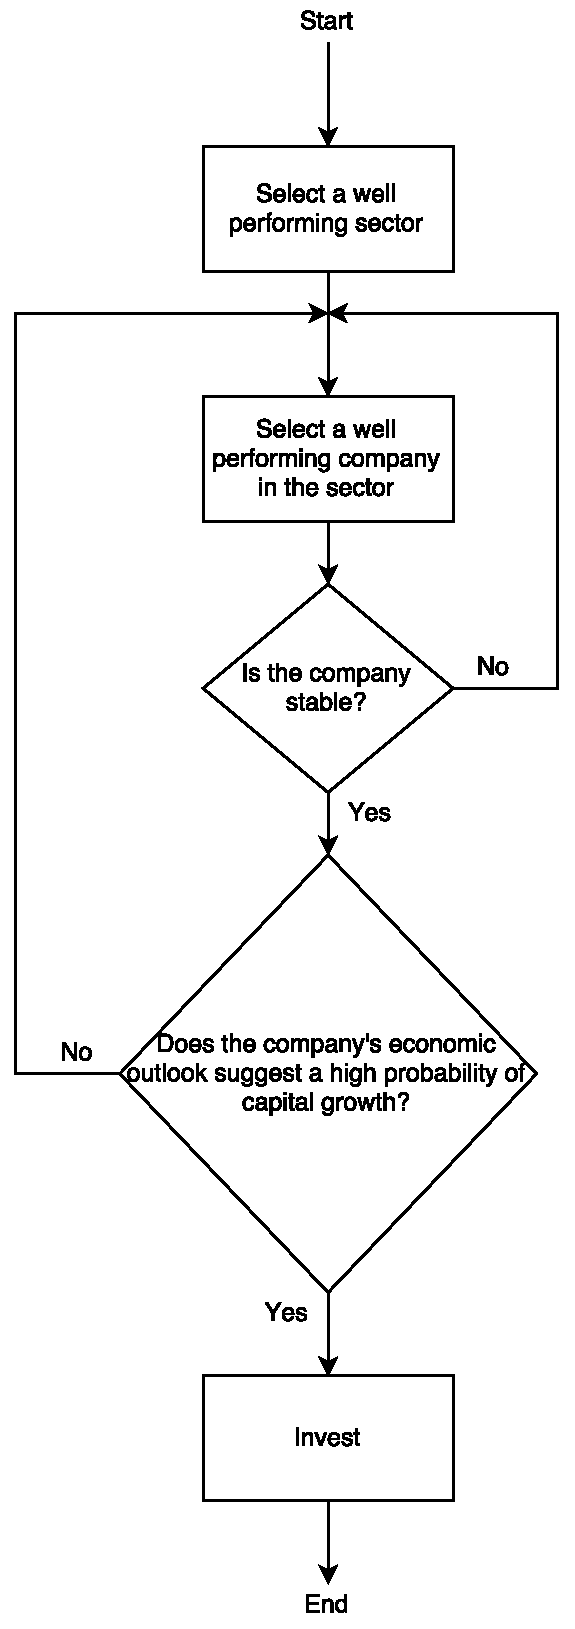
\includegraphics[scale=0.5]{decisions.pdf}
\caption{Flow diagram of investment selection}
\label{fig:flowChart}
\end{figure}

\label{sec:flowChart}



\bibliographystyle{plain}
\bibliography{bib} 



\end{document}
